
\documentclass[25pt, portrait,  margin=0mm, innermargin=15mm,
  blockverticalspace=15mm, colspace=15mm, subcolspace=8mm]{tikzposter}



\usepackage[utf8]{inputenc}

\usetheme{Basic}

\makeatletter
\setlength{\TP@visibletextwidth}{225cm}
\setlength{ \TP@visibletextheight}{120cm}
\makeatother

\title{FemtoGraph: A Pregel Based Multithreaded
  Graph Processing Library}

\author{
  \textbf{Alex Ballmer}\\
  \textit{Illinois Institute of Technology}\\
  alexandersballmer@gmail.com\\
  \textbf{Ioan Raicu}\\
  \textit{Illinois Institute of Technology}\\
  iraicu@cs.iit.edu\\
}


\geometry{paperwidth=243.84cm,paperheight=121.92cm}


\begin{document}

\maketitle

\begin{columns}
    \column{0.25}
    \block[roundedcorners=40]{Abstract} {


  The emerging applications for large graphs in big data science and social networks has led to the development of numerous parallel or distributed graph processing applications. The need for faster manipulation of graphs has driven the need to scale accross large core counts and many parallel machines. While distributed memory parallel systems continue to be used for high performance computing, some smaller systems make use of shared memory (SMP) and larger core counts. I hope to explore ways to utilize these larger shared memory systems by implementing a framework for manipulating graphs at a large scale. This system should be able to leverage and scale to very large core counts and provide a framework for later incorporating distributed processing across multiple nodes.
}


    \block[roundedcorners=40]{Related Work} {
      \textbf{Other Graph Processing Systems}\par
      The field of graph processing is very well defined with many existing commercial and opensource applications and tools available.
      \begin{itemize}
      \item \textbf{GraphLab} Single node or parallel asynchronous vertex-centric framework 
      \item \textbf{Hadoop} MapReduce based parallel framework using hdfs filesystem. While not designed for graph processing alone, a graph processing algorithm can be thought of as a series of chained MapReduce functions
      \item \textbf{Apache Spark} MapReduce based parallel framework faster than Hadoop with in-memory processing 
      \item \textbf{Apache Giraph} Application on top of Hadoop for dedicated graph processing
      \end{itemize}

      \textbf{Comparing Application Performance}\par
      We chose to use GraphLab as a reference point to judge application performance as it is designed to run in a shared memory configuration on a single node. 
      }

    \block[roundedcorners=40]{Pregel Model} {
      FemtoGraph is based off of the Pregel Model of graph processing

      \begin{itemize}
      \item Vertex-centric: \textit{think like a vertex}
      \item Computation occurs in synchronous \textit{supersteps}
      \item \textit{Compute function} called in parallel in the context of each vertex
      \item All compute functions must be called before next superstep
      \item Vertices can update edges and neighboring vertices
      \item Vertices can send messages to vertices in the \textit{next} superstep only
      \item Vertices can \textit{vote to halt}. Vertices un-halt upon receiving a message
      \item When all vertices are halted, the simulation ends
      \end{itemize}
      
      }

    \block[roundedcorners=40]{Implementation} {

      \begin{itemize}
      \item Written in C++ with Boost libraries
      \item Graph stored in adjacency list
      \item Message queue based on multiple Boost lockfree queues
      \item Uses normal std::thread for multithreading.
      \item Compute function is a user defined function run in the context of each vertex
      \item Compute functions are called in parallel
      \end{itemize}


    }
    \column{0.25}
    \block[roundedcorners=40]{Initial Problems} {
      \textbf{Initial FemtoGraph could not scale past 4 cores}
      \begin{itemize}
      \item  Very bad scaling
      \item Tried various graph storage techniques and threading patterns
      \item Little improvement
      \end{itemize}
      \setcounter{figurecounter}{98}
      \begin{tikzfigure}[Less than perfect scaling\label{test_lable}]
        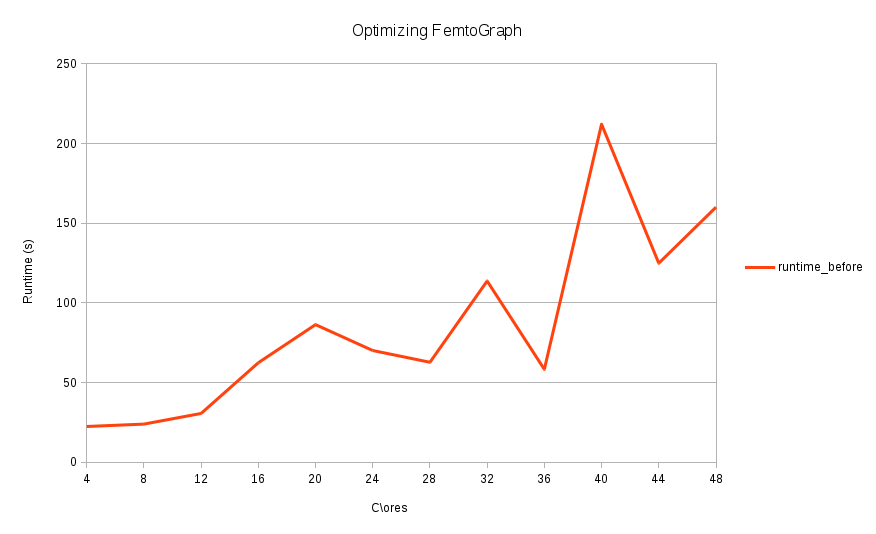
\includegraphics[width=0.65\linewidth]{before.png}
      \end{tikzfigure}
      \begin{itemize}
      \item Initial message queue used global mutexes (not lockfree) 
      \item Profiling using callgrind showed bottleneck in message queue
      \end{itemize}
      \setcounter{figurecounter}{98}
      \begin{tikzfigure}[Callgrind profiling]
        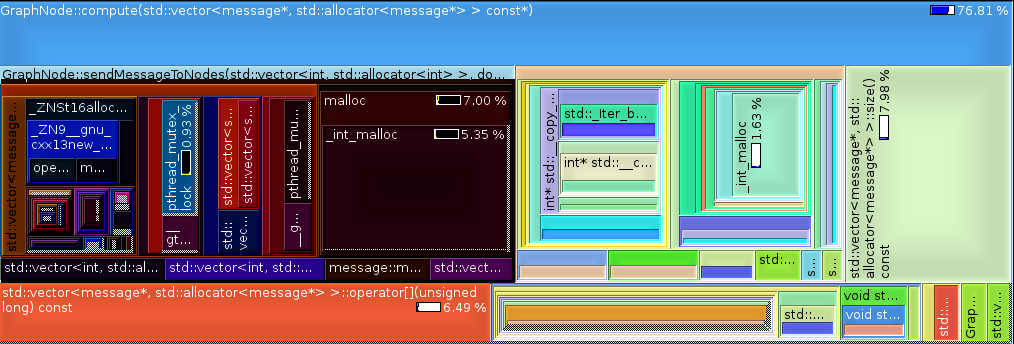
\includegraphics[width=0.85\linewidth]{callgrind.png}
      \end{tikzfigure}
      \begin{itemize}
      \item Highlighted area shows message queue blocking until mutex is freed
      \end{itemize}


      }
    
    \block[roundedcorners=40]{Final Results} {
      \setcounter{figurecounter}{98}
      \begin{tikzfigure}[Scaling vs GraphLab\label{test_lable}]
        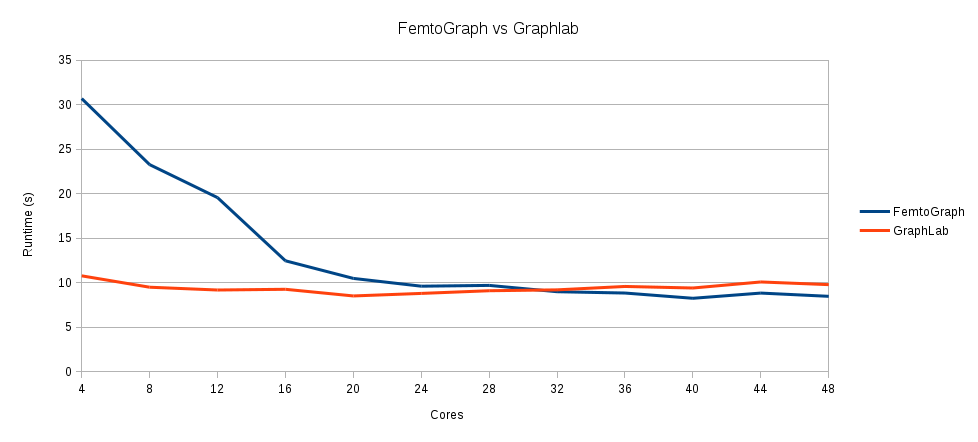
\includegraphics[width=0.95\linewidth]{vs.png}
        \end{tikzfigure}


      }

    
\end{columns}
\end{document}
